\documentclass{article}
\usepackage[utf8]{inputenc}
\usepackage{caption}
\usepackage{empheq}
\usepackage{siunitx}
\usepackage{booktabs}
\usepackage{pgfplots}
\usepackage{graphicx}
\usepackage{hyperref}
\usepackage{tabularx}
\usepackage{makecell}

\setlength{\parindent}{0pt}

\newcommand{\answer}[1]{\begin{center}\boxed{#1}\end{center}}
\newcommand{\degree}{$^{\circ}$}

\newenvironment{changemargin}[2]{%
\begin{list}{}{%
\setlength{\topsep}{0pt}%
\setlength{\leftmargin}{#1}%
\setlength{\rightmargin}{#2}%
\setlength{\listparindent}{\parindent}%
\setlength{\itemindent}{\parindent}%
\setlength{\parsep}{\parskip}%
}%
\item[]}{\end{list}}

\title{Determining the Wavelength of a Laser using Interferometry Techniques}
\author{Maxwell Fan}
\date{January 2020}

\begin{document}

\maketitle

\section*{\centering{Abstract}}

\begin{center}
    %\begin{changemargin}{0.3cm}{0.3cm}
        \begin{flushleft}

            Lasers emit light at a very specific frequency and wavelength. With knowledge of the specific frequency and wavelength, it is possible to measure distances to a very high degree of accuracy (within one-half the wavelength). However, there are few simple ways to accurately measure the wavelength of a laser. 
            Most methods utilize an interferometer, taking advantage of the wave nature of light and the phenomenon of wave interference. 
            The standard procedure for measuring the wavelength of a laser using an interferometer would normally require many hours of manual fringe counting to achieve accurate results with a reasonable standard deviation.
            But, using an interferometer and automatic fringe counting, we implement and demonstrate a more accurate and rapid method for determining the wavelength of a laser.

        \end{flushleft}
    %\end{changemargin}
\end{center}

\bigskip
\bigskip

\section*{Introduction}
Thomas Young, in his 1801 paper on the wave nature of light, demonstrated that light can constructively and destructively interfere with itself. Utilizing the double-slit interference patterns  of light, he demonstrated that light is both a wave and a particle. This concept has been extended to an interferometer, which accurately measures the distance in path length ($\Delta p$) in a split beam of light. By relying on the unique properties of light, rather than a comparison to a known object, such as a meter stick, the interferometer is able to achieve higher accuracy and precision.

\bigskip
\begin{figure}[!ht]
\begingroup
    \rightskip
    \leftskip
    \begin{center}
        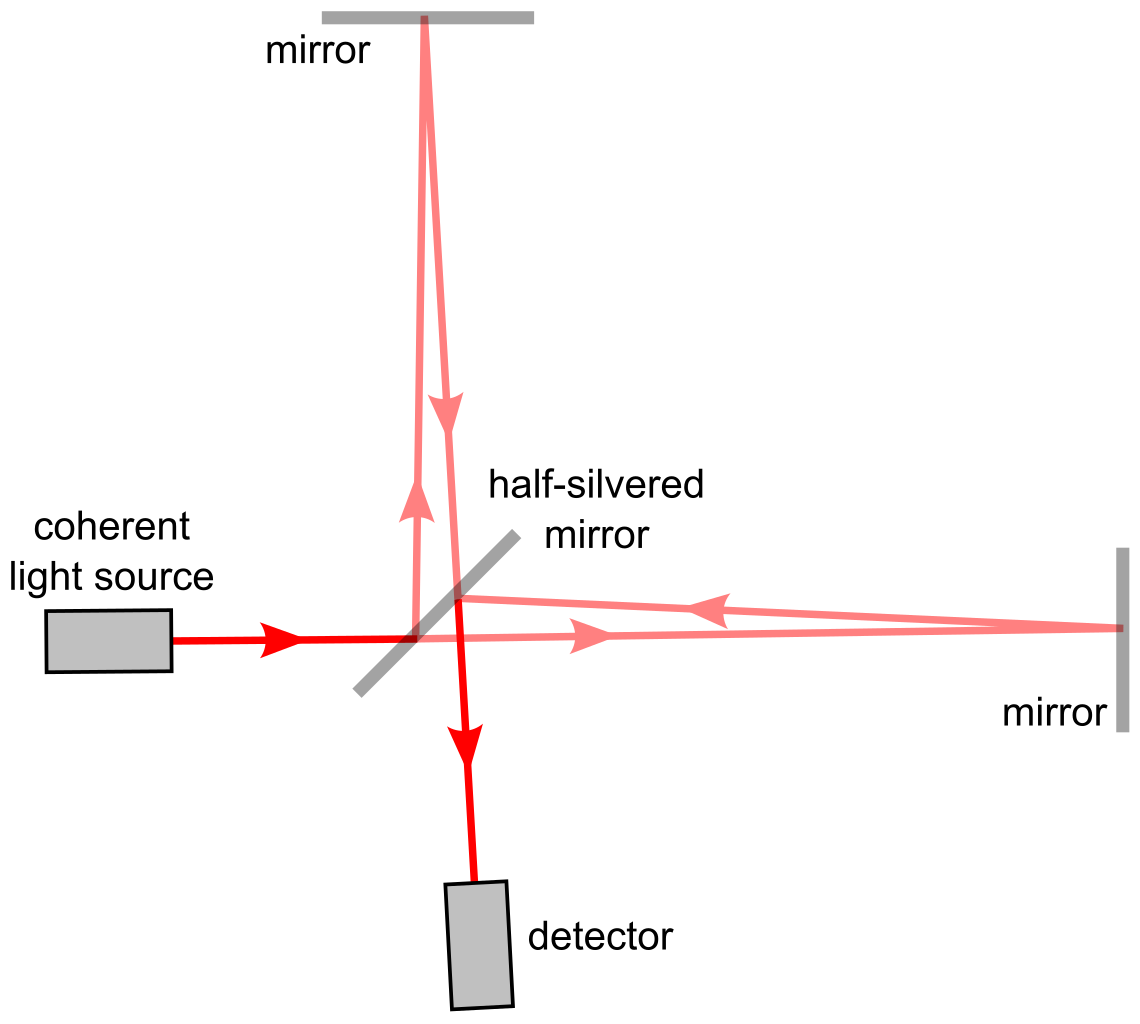
\includegraphics[width=300pt,height=270pt]{interferometer.png}
        \caption*{Figure 1. A typical interferometer setup that generates circular, concentric fringes.}
    \end{center}
\endgroup
\end{figure}

There are two types of interferometers that generate distinct interference patterns, depending on the orientation of the mirrors. If both mirrors are neither perpendicular nor parallel to the light source, they will generate hyperbolic fringes. If both mirrors are perpendicular or parallel to the light source, they will generate circular, concentric fringes, as shown in Figure 1.

\bigskip

Regardless of the fringe pattern produced by the interferometer, varying the difference in the path length traveled by the two separated beams changes fringe patterns. When varying the path length, each antinode is one $\lambda$ apart, so increasing the path length by one $\lambda$ will result in the formation of a identical interference pattern (with each node shifted over by one). Since light travels back and forth from the mirror, changing $\Delta d$, the difference in distance from each mirror to the beam splitter, by one micron, will result in $\Delta p$, the light path changing by two microns.

\bigskip

By counting the number of fringes that appear when moving the micrometer by a known distance, the wavelength of the laser can be determined. Given $\Delta d$, the change in mirror distance from the beam splitter in microns, and $n$, the number of fringes, the wavelength $\lambda$ is, in nanometers is:

\begin{center}
    $\lambda = \frac{\Delta d \times 2000}{n}$
\end{center}

\section*{Methods}

\begin{figure}[!ht]
\begingroup
    \rightskip
    \leftskip
    \begin{center}
        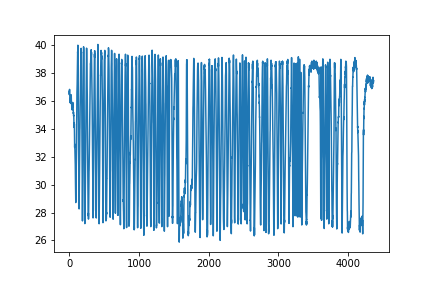
\includegraphics[width=300pt,height=200pt]{4_raw.png}
        \caption*{Figure 2. Initial graph of average brightness of the bounding box over frames taken in trial 4.}
    \end{center}
\endgroup
\end{figure}

\begin{figure}[!ht]
\begingroup
    \rightskip
    \leftskip
    \begin{center}
        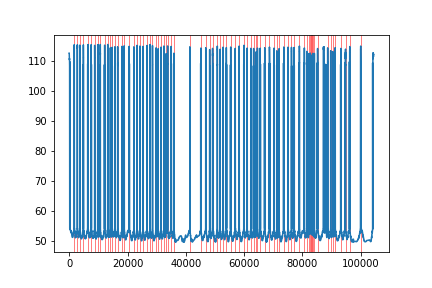
\includegraphics[width=300pt,height=200pt]{4_final.png}
        \caption*{Figure 3. Final graph of transformed and dilated brightness of the bounding box over frames taken with detected peaks highlighted in trial 4.}
    \end{center}
\endgroup
\end{figure}
After varying the micrometer, which controls the distance ($\Delta d$) between the beam splitter and the mirror, each fringe was captured using a slow-motion camera at a high frame rate, allowing for rapid computational counting. This allow more data to be collected and analyzed in the short 20 minutes of allotted data collection time provided for the elliptical interferometer. Since the pattern on the wall can be thought of as a wave of brightness traveling from the central antinode outwards, the graph of brightness at a specific point should also be approximately the same wave pattern as the interference pattern. Using this principle, for each slow-motion video captured, a bounding box was created roughly over the central antinode, and the average aggregate brightness of the R, G, and B channels in the box was graphed over time. Once the data was converted to a graph of average brightness values (Figure 2), the graph was aggressively dilated to exaggerate the peaks, translated to have a smoother moving average, and values below the moving average were double-counted to increase the prominence of each peak (Figure 3). After each peak was detected, it was manually reviewed by an eyeball check to ensure that no peaks were double-counted and to manually account for the cut-off of the first and last peaks.

\bigskip

In trial 4, the algorithm counted 78 peaks (Figure 3), however, it missed a peak at approximately 90000 and did not include the first and last peaks, due to them being partially cut off. Therefore, three peaks were manually added to the peak count, bringing the total number of peaks up to 81.

\bigskip

% Using OpenCV, a popular Python computer vision library, an automated fringe counting mechanism was developed.  


\section*{Results}
Out of the 17 trials where data was collected and analyzed, three of them were dropped. The first trial was dropped due to the poor data quality that the circle interference pattern generated; no other analyzed trial used the circle interferometer. The third trial was dropped due to poor record-keeping, as it was unclear if the micrometer was actually moved by exactly 100 microns. Finally, the 16th trial was dropped due to an accidential overshoot of the dial, which led to double-counting several fringes. 

% TODO: ensure figure number is accurate 
\begin{table}[!ht]
\centering
\captionsetup{labelformat=empty}
\caption{Figure 4. Table of Fringe Counting Results}
\begin{tabular}{llll}
Trial \#           & Count & Length (microns) & Wavelength (nm)  \\ 
\hline
1*                 & 72    & 25               & 694.4444444      \\ 
\hline
2                  & 77    & 25               & 649.3506494      \\ 
\hline
3*                 & 285   & 100              & 701.754386       \\ 
\hline
4                  & 81    & 25               & 617.2839506      \\ 
\hline
5                  & 76.5  & 25               & 653.5947712      \\ 
\hline
6                  & 76    & 25               & 657.8947368      \\ 
\hline
7                  & 81    & 25               & 617.2839506      \\ 
\hline
8                  & 80    & 25               & 625              \\ 
\hline
9                  & 80    & 25               & 625              \\ 
\hline
10                 & 79    & 25               & 632.9113924      \\ 
\hline
11                 & 82    & 25               & 609.7560976      \\ 
\hline
12                 & 78    & 25               & 641.025641       \\ 
\hline
13                 & 78    & 25               & 641.025641       \\ 
\hline
14                 & 77    & 25               & 649.3506494      \\ 
\hline
15                 & 79    & 25               & 632.9113924      \\ 
\hline
16*                & 86    & 25               & 581.3953488      \\ 
\hline
17                 & 78    & 25               & 641.025641       \\
                   &       &                  &                  \\
Mean               &       &                  & 635.2438938      \\ 
\hline
Standard Deviation &       &                  & 14.84174213     
\end{tabular}
\end{table}

\bigskip

From the results, we can determine that the wavelength of the unknown laser is likely $635 \pm 15 \si{\nano\meter}$, assuming that it is within one standard deviation of the measurements (Figure 4).

\section*{Discussion}
Our data seems quite reasonable, and are mostly within the expected wavelengths for red light. However, since the same peak-counting mechanism was used for all data collected, the entire dataset may be consistently skewed to either undercount or overcount peaks. 
To prevent this bias from occurring, 10-30 peaks from each trial was randomly sampled and manually counted to increase confidence in the peak counting mechanism. Nonetheless, randomly sampling the peak counts consumed the majority of the analysis time and did intially catch a few uncounted peaks and resulted in tweaks to the peak counting mechanism. 
But, once the fringe-counting process was mostly automated, it took, on average, one minute to capture the data and 5-10 minutes to process each slow-motion video, a significant improvement on manual counting. 

\bigskip

Furthermore, an attempt was made to automate the initial pre-processing stage, which consisted of cutting and cropping the footage. This was attempted by iteratively removing outer rows and columns that had an average brightness below a threshold percent of the total average brightness. However, this was found to be an unreliable method of cropping regions since some footage contained reflections of the sun. Future work may attempt to subtract the blue and green channels from the red channels to eliminate white colors, rather than aggregating the three channels.

\bigskip

With the circle-patterned interferometer, it was more difficult to get reliable data since, at times, fringes blurred with each other due to the glare and the averaging box always capturing portions of multiple fringes, which reduced the prominence of the brightness peaks during analysis.
Unfortunately, our implementation of circle hough transform (CHT) from the literature could not reliably detect the noisy circle-patterned fringes. If a proper circle detection algorithm was implemented, however, it would be significantly easier to filter out noise. In the future, more flexible circle detection algorithms or better pre-processing techniques may increase the quality of the footage from the circle-patterned interferometer. Additionally, future attempts to speed up and refine the methods described may focus on trying to create a one-size-fits all algorithm for automatic peak detection of sinusoidal data, rather than manually setting parameters. 

\end{document}
